\section{TinyDAS}
\label{res:tinydas}

In this section, we'l be looking at the results for both training our autoencoders, as well as testing our models on the test data mentioned in the method section.




\subsection{Experiment 1: Model training}

As we can see in the table ...

\begin{table}[!htbp]
\centering
%\small
\begin{tabular}{@{}l*{4}{l}@{}}
\toprule
\textbf{Parameter} & \textbf{AE} & \textbf{VAE} & \textbf{CAE} & \textbf{CVAE}\\
\midrule
Files & \multicolumn{4}{c}{25600} \\
Input Shape & \multicolumn{4}{c}{$625 \times 2137$} \\
Validation Split & \multicolumn{4}{c}{0.2} \\
Epochs & \multicolumn{4}{c}{100} \\
Batch Size & 512 & 512 & 64 & 64 \\
Optimizer & \multicolumn{4}{c}{ADAM} \\
Learning rate & \multicolumn{4}{c}{0.0001} \\
Loss function & \acrshort{mse} & \acrshort{elbo} & \acrshort{mse} & \acrshort{elbo} \\
Layer sizes & \multicolumn{2}{c}{$[1024, 512, 128, 64]$}  & \multicolumn{2}{c}{[1, 16, 8, 8]}\\
Latent dim & \multicolumn{4}{c}{32} \\
Datatype & FP16 & FP32 & FP16 & FP32 \\
Model Sizes (\si{\giga\byte})& 2.71 & \textbf{0.00001159} & 5.183 & 0.335 \\
%Dropout (p) & \multicolumn{4}{c}{0.0} \\
Early stopping patience & \multicolumn{4}{c}{5} \\
Early stopping min delta & \multicolumn{4}{c}{0.000005} \\
\bottomrule
\end{tabular}
\caption{Hyperparameters for all models}
\label{tab:hyperparameters}
\end{table}


\begin{table}[!htbp]
    \centering
    \begin{tabular}{lcccc}
        \hline
        \textbf{Metric} & \textbf{AE} & \textbf{CAE} & \textbf{VAE} & \textbf{CVAE} \\
        \hline
        Best loss & 1.3e-6 & 0.032 & 0.038 & 0.029 \\
        Epochs before stop & 6 & 20 & 15 & 15 \\
        \hline
    \end{tabular}
    \caption{Comparison of Autoencoder Performance\\ *The Reconstruciton error is the sum of all reconstruction errors across all batches.}
    \label{tab:autoencoder_comparison}
\end{table}

\begin{figure}[!h]
    \centering
    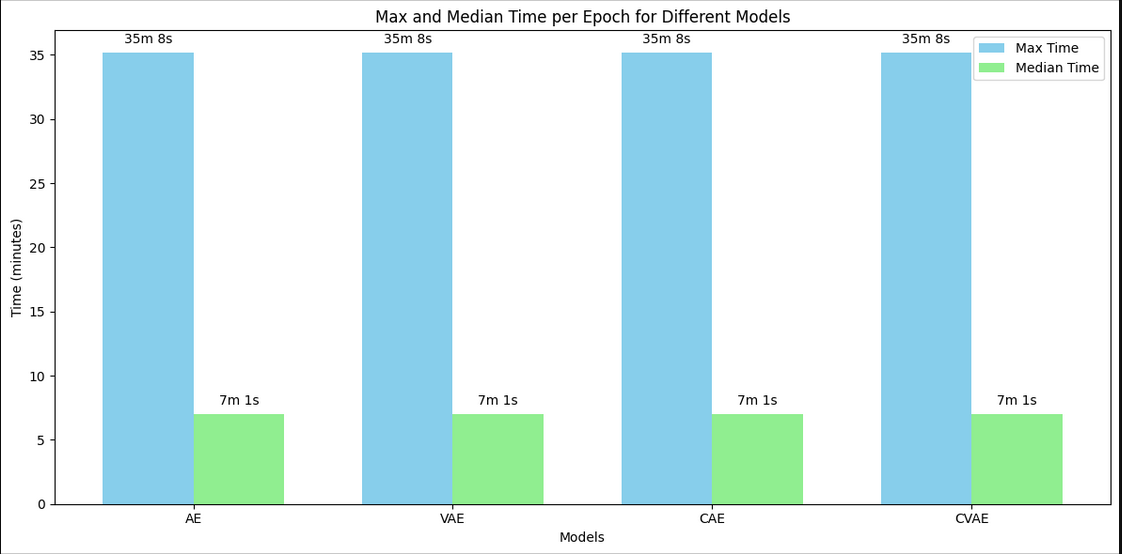
\includegraphics[scale=0.4]{figures/time.png}
    \caption{Training times}
    \label{fig:traintimes}
\end{figure}

As we can see in figure \ref{fig:traintimes}, there is a huge difference between the max training time and the median training time. The max training time always happens during the first epoch, when the \texttt{train\_step} and \texttt{val\_step} kernels are being compiled. Total training times per model are all under \qty{6}{\si{\hour}} before the training is stopped early due to the \textit{early stopping} mechanism.

\subsubsection{Loss Values}

The following is a list of how the losses changed over time...


\begin{figure}[!htbp]
  \centering
  \begin{subfigure}[t]{.6\textwidth}
    \centering
    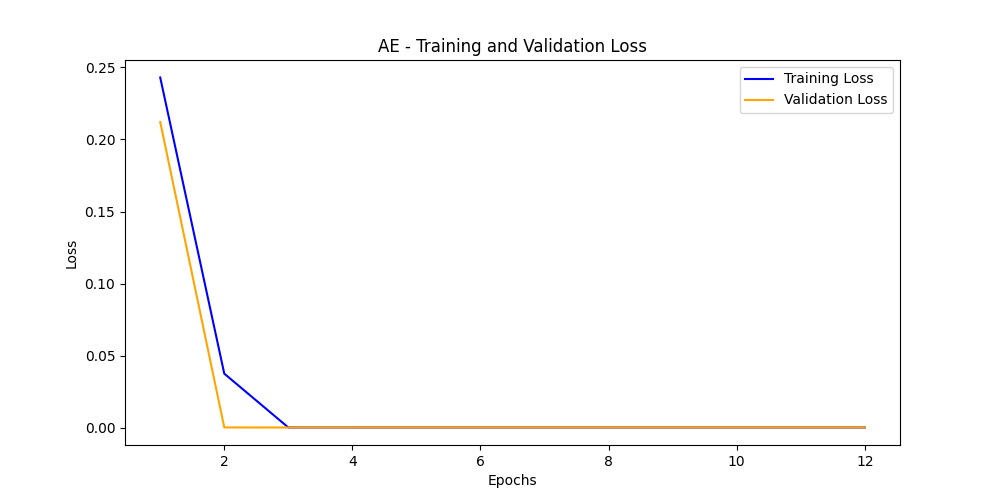
\includegraphics[width=\linewidth]{figures/losses/ae.png}
    \caption{AE}
  \end{subfigure}
  \hfill
  \begin{subfigure}[t]{.6\textwidth}
    \centering
    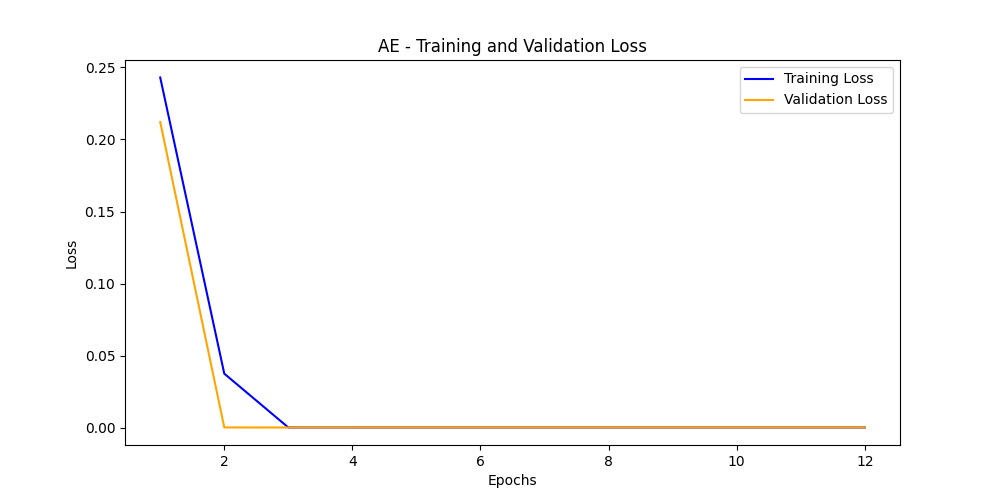
\includegraphics[width=\linewidth]{figures/losses/ae.png}
    \caption{CAE}
  \end{subfigure}
  
  \vspace{1cm}
  
  \begin{subfigure}[t]{.6\textwidth}
    \centering
    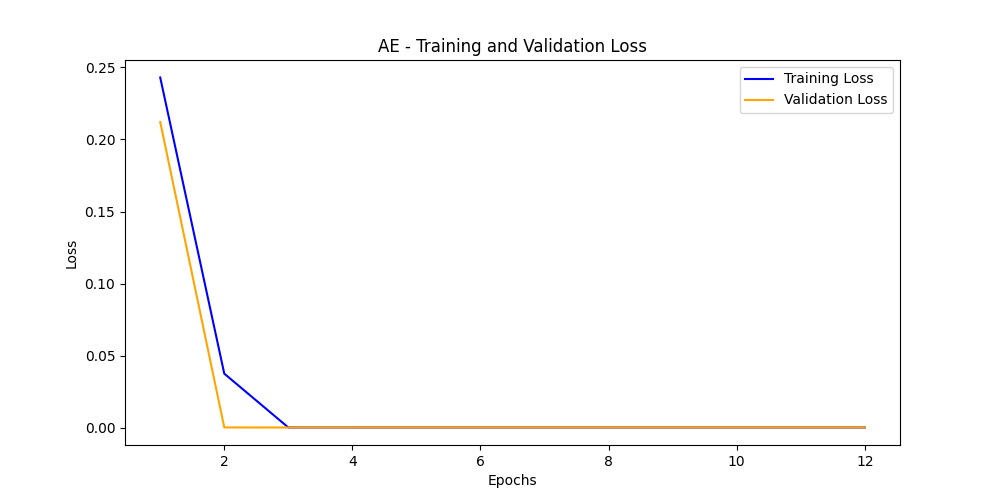
\includegraphics[width=\linewidth]{figures/losses/ae.png}
    \caption{VAE}
  \end{subfigure}
  \hfill
  \begin{subfigure}[t]{.6\textwidth}
    \centering
    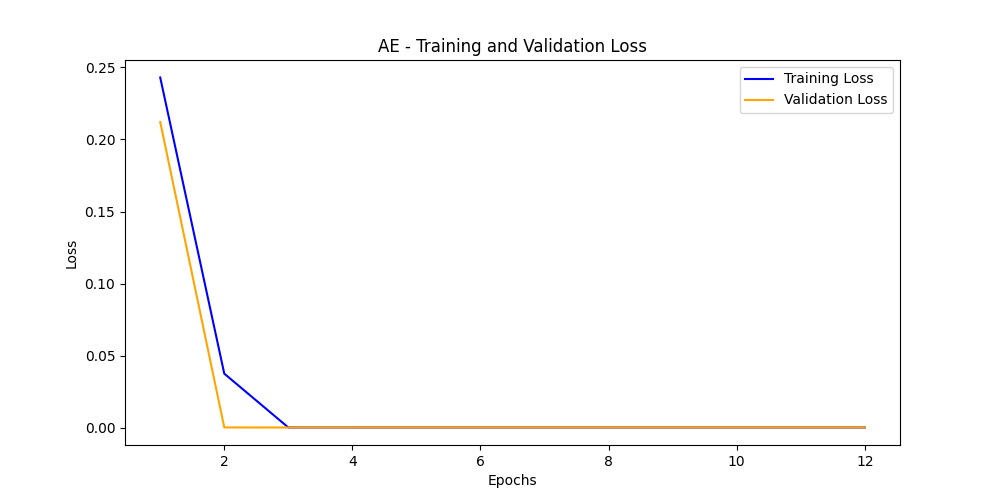
\includegraphics[width=\linewidth]{figures/losses/ae.png}
    \caption{CVAE}
  \end{subfigure}
  \caption{Train and Validation Loss per epoch}
\end{figure}

\subsubsection{Reconstruction Capabiltites}

\begin{figure}[!h]
    \centering    
    % Row 0 (Image Names)
    \begin{subfigure}{0.33\textwidth}
        \centering
        \textbf{Image 1}
    \end{subfigure}%
    \hfill
    \begin{subfigure}{0.33\textwidth}
        \centering
        \textbf{Image 2}
    \end{subfigure}%
    \hfill
    \begin{subfigure}{0.33\textwidth}
        \centering
        \textbf{Image 3}
    \end{subfigure}
    
    \vspace{1em}
    
    % Row 1 (Original)
    \begin{subfigure}{0.33\textwidth}
        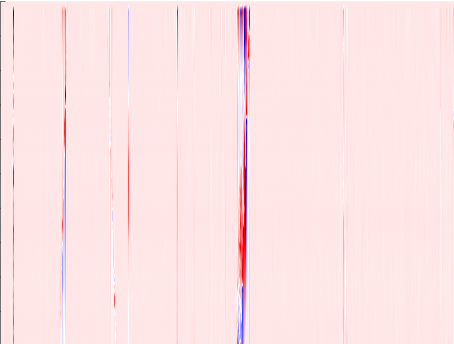
\includegraphics[width=\textwidth]{figures/test.png}
        \caption{Original}
    \end{subfigure}%
    \hfill
    \begin{subfigure}{0.33\textwidth}
        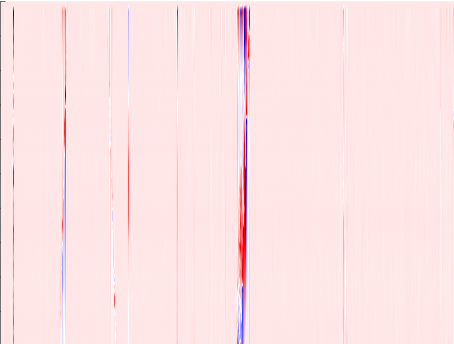
\includegraphics[width=\textwidth]{figures/test.png}
        \caption{Original}
    \end{subfigure}%
    \hfill
    \begin{subfigure}{0.33\textwidth}
        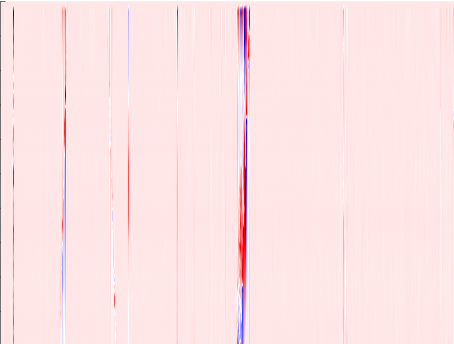
\includegraphics[width=\textwidth]{figures/test.png}
        \caption{Original}
    \end{subfigure}
    
    \vspace{1em}
    
    % Row 2 (Model 1)
    \begin{subfigure}{0.33\textwidth}
        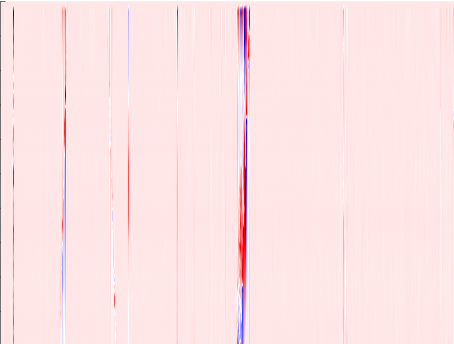
\includegraphics[width=\textwidth]{figures/test.png}
        \caption{AE}
    \end{subfigure}%
    \hfill
    \begin{subfigure}{0.33\textwidth}
        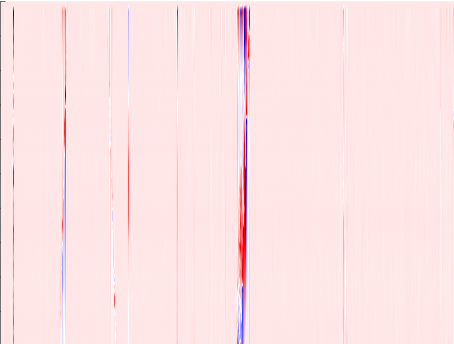
\includegraphics[width=\textwidth]{figures/test.png}
        \caption{AE}
    \end{subfigure}%
    \hfill
    \begin{subfigure}{0.33\textwidth}
        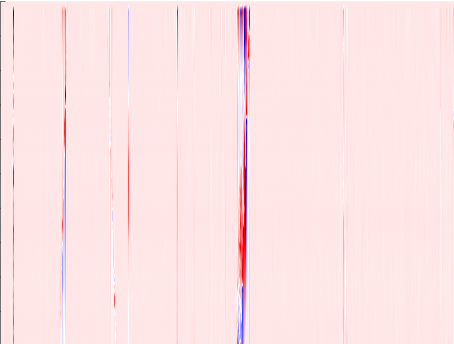
\includegraphics[width=\textwidth]{figures/test.png}
        \caption{AE}
    \end{subfigure}
    
    \vspace{1em}
    
    % Row 3 (Model 2)
    \begin{subfigure}{0.33\textwidth}
        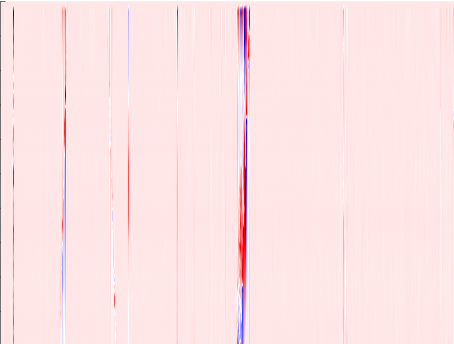
\includegraphics[width=\textwidth]{figures/test.png}
        \caption{CAE}
    \end{subfigure}%
    \hfill
    \begin{subfigure}{0.33\textwidth}
        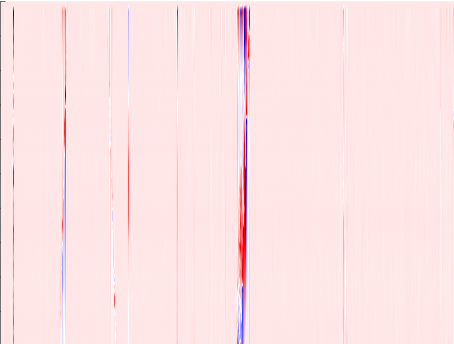
\includegraphics[width=\textwidth]{figures/test.png}
        \caption{CAE}
    \end{subfigure}%
    \hfill
    \begin{subfigure}{0.33\textwidth}
        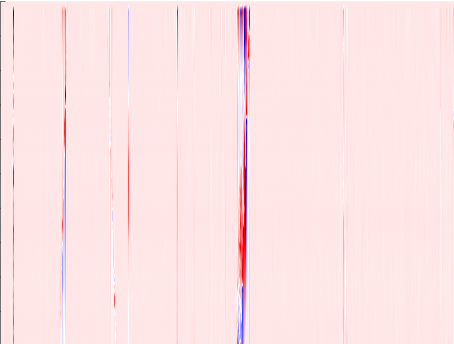
\includegraphics[width=\textwidth]{figures/test.png}
        \caption{CAE}
    \end{subfigure}
    
    \vspace{1em}
    
    % Row 4 (Model 3)
    \begin{subfigure}{0.33\textwidth}
        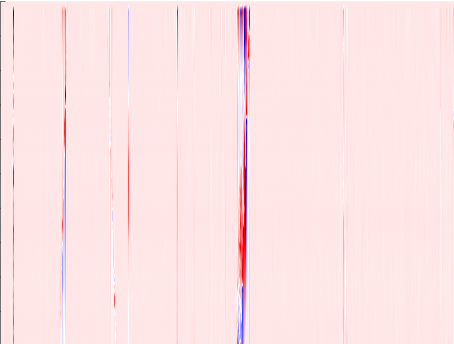
\includegraphics[width=\textwidth]{figures/test.png}
        \caption{VAE}
    \end{subfigure}%
    \hfill
    \begin{subfigure}{0.33\textwidth}
        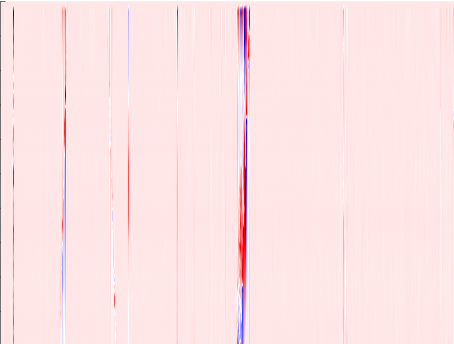
\includegraphics[width=\textwidth]{figures/test.png}
        \caption{VAE}
    \end{subfigure}%
    \hfill
    \begin{subfigure}{0.33\textwidth}
        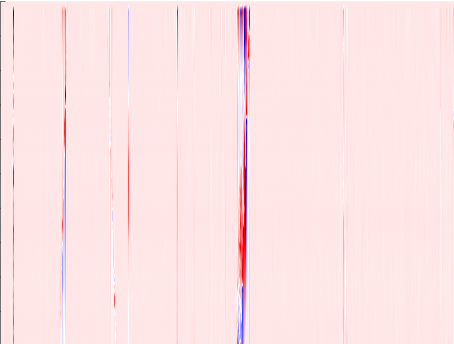
\includegraphics[width=\textwidth]{figures/test.png}
        \caption{VAE}
    \end{subfigure}
    
    \vspace{1em}
    
    % Row 5 (Model 4)
    \begin{subfigure}{0.33\textwidth}
        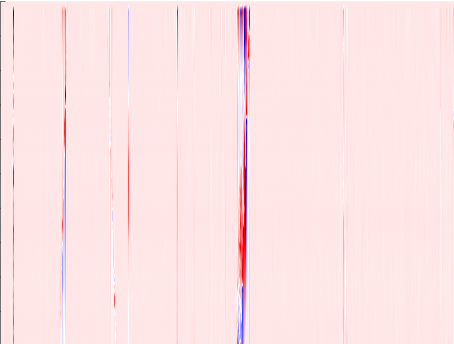
\includegraphics[width=\textwidth]{figures/test.png}
        \caption{CVAE}
    \end{subfigure}%
    \hfill
    \begin{subfigure}{0.33\textwidth}
        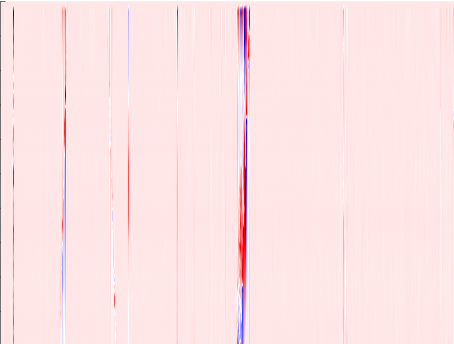
\includegraphics[width=\textwidth]{figures/test.png}
        \caption{CVAE}
    \end{subfigure}%
    \hfill
    \begin{subfigure}{0.33\textwidth}
        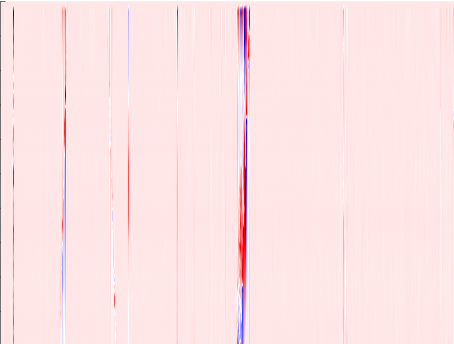
\includegraphics[width=\textwidth]{figures/test.png}
        \caption{CVAE}
    \end{subfigure}
    
    \caption{Comparison of original images and their reconstructions by different autoencoders}
    \label{fig:aereconstruct}
\end{figure}

\subsection{Autoencoder Performance Comparison}

An important part of analysing our autoencoders is the choice of metrics. Whereas loss and accuracy can provide proficient details about the model training itself, other metrics are better suited for analysing the 

Table \ref{tab:autoencoder_comparison} presents a comparative analysis of the four autoencoder types: dense, convolutional, variational dense, and variational convolutional.



\subsection{Performance Visualization}


% Confusion Matrix Components Table
\begin{table}[!htbp]
\centering
\label{tab:confusion-matrix-results}
\begin{tabular}{l
    S[table-format=3.0]
    S[table-format=3.0]
    S[table-format=3.0]
    S[table-format=3.0]
    S[table-format=3.2]
    S[table-format=3.2]
}
\toprule
\textbf{Model} & {\textbf{TP}} & {\textbf{FP}} & {\textbf{TN}} & {\textbf{FN}} & {\textbf{Precision (\%)}} & {\textbf{Recall (\%)}} \\
\midrule
\rowcolor{gray!10} AE   & 100 & 10 & 80 & 10 & 90.91 & 90.91 \\
CAE  & 95 & 15 & 75 & 15 & 86.36 & 86.36 \\
\rowcolor{gray!10} VAE  & 105 & 8 & 85 & 5 & 92.92 & 95.45 \\
CVAE & 30 & 110 & 460 & 0 & 21.43 & 100.00 \\
\bottomrule
\end{tabular}
\caption{Confusion Matrix Components and Derived Metrics}
\end{table}


% Performance Metrics Table

\begin{table}[!htbp]
\centering
\label{tab:performance-metrics}
\begin{tabular}{l
    S[table-format=1.3]
    S[table-format=1.3]
    S[table-format=1.3]
    S[table-format=1.3]
    S[table-format=1.3]
}
\toprule
\textbf{Model} & {\textbf{TPR}} & {\textbf{FPR}} & {\textbf{Precision}} & {\textbf{F1-Score}} & {\textbf{Accuracy}} \\
\midrule
\rowcolor{gray!10} AE   & 0.909 & 0.111 & 0.909 & 0.909 & 0.900 \\
CAE  & 0.864 & 0.167 & 0.864 & 0.864 & 0.850 \\
\rowcolor{gray!10} VAE  & 0.955 & 0.086 & 0.929 & 0.942 & 0.941 \\
CVAE & 0.910 & 0.128 & 0.910 & 0.900 & 0.817 \\
\bottomrule
\end{tabular}
\caption{Model Performance Metrics Comparison}
\end{table}

\begin{figure}[!h]
\centering
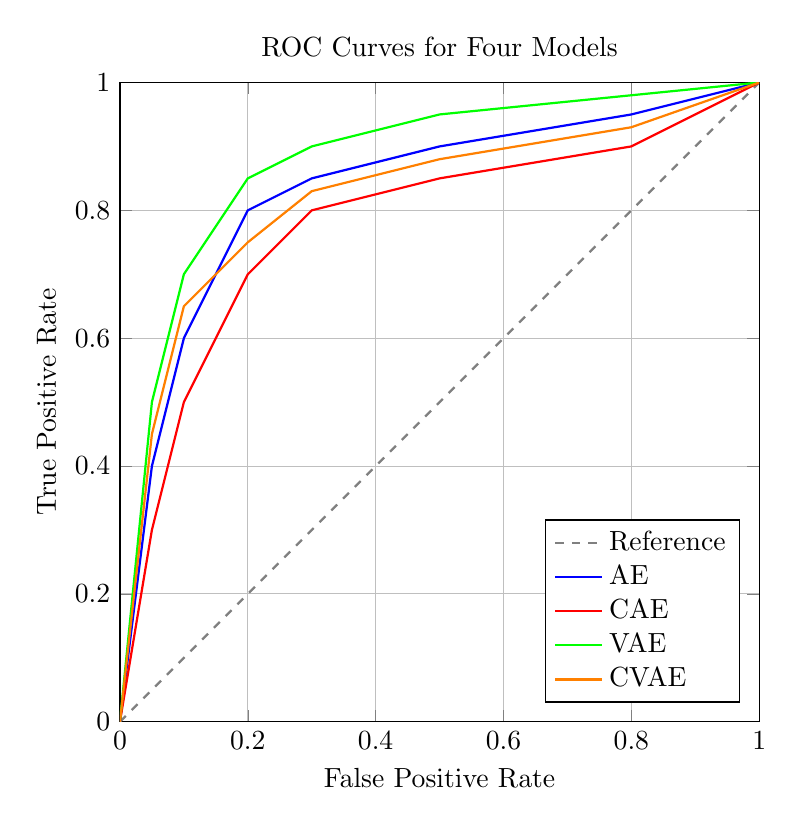
\begin{tikzpicture}
\begin{axis}[
    width=0.8\textwidth,
    height=0.8\textwidth,
    xlabel={False Positive Rate},
    ylabel={True Positive Rate},
    xmin=0, xmax=1,
    ymin=0, ymax=1,
    xtick={0,0.2,0.4,0.6,0.8,1},
    ytick={0,0.2,0.4,0.6,0.8,1},
    legend pos=south east,
    legend cell align={left},
    grid=major,
    title={ROC Curves for Four Models}
]

% Diagonal reference line
\addplot[thick,dashed,gray] coordinates {(0,0) (1,1)};

% ROC curve for Model A
\addplot[thick,blue] coordinates {
    (0,0) (0.05,0.4) (0.1,0.6) (0.2,0.8) (0.3,0.85) (0.5,0.9) (0.8,0.95) (1,1)
};

% ROC curve for Model B
\addplot[thick,red] coordinates {
    (0,0) (0.05,0.3) (0.1,0.5) (0.2,0.7) (0.3,0.8) (0.5,0.85) (0.8,0.9) (1,1)
};

% ROC curve for Model C
\addplot[thick,green] coordinates {
    (0,0) (0.05,0.5) (0.1,0.7) (0.2,0.85) (0.3,0.9) (0.5,0.95) (0.8,0.98) (1,1)
};

% ROC curve for Model D
\addplot[thick,orange] coordinates {
    (0,0) (0.05,0.45) (0.1,0.65) (0.2,0.75) (0.3,0.83) (0.5,0.88) (0.8,0.93) (1,1)
};

\legend{Reference, AE, CAE, VAE, CVAE}

\end{axis}
\end{tikzpicture}
\caption{ROC Curves Comparison for our Autoencoders }
\end{figure}

\begin{figure}[!h]
\centering
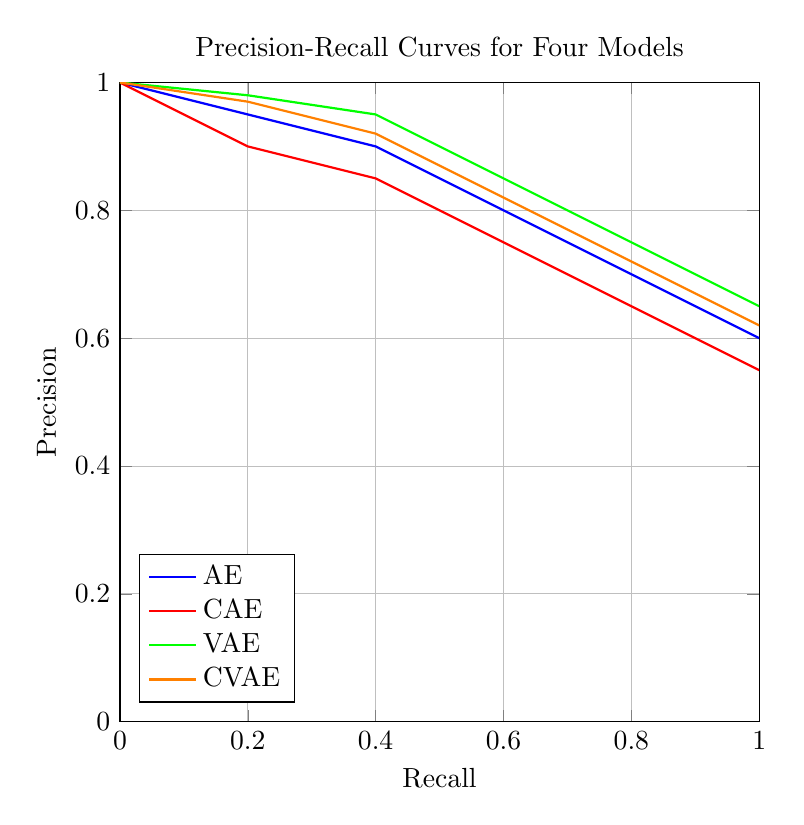
\begin{tikzpicture}
\begin{axis}[
    width=0.8\textwidth,
    height=0.8\textwidth,
    xlabel={Recall},
    ylabel={Precision},
    xmin=0, xmax=1,
    ymin=0, ymax=1,
    xtick={0,0.2,0.4,0.6,0.8,1},
    ytick={0,0.2,0.4,0.6,0.8,1},
    legend pos=south west,
    legend cell align={left},
    grid=major,
    title={Precision-Recall Curves for Four Models}
]
% PR curve for Model AE
\addplot[thick,blue] coordinates {
    (0,1) (0.2,0.95) (0.4,0.9) (0.6,0.8) (0.8,0.7) (1,0.6)
};
% PR curve for Model CAE
\addplot[thick,red] coordinates {
    (0,1) (0.2,0.9) (0.4,0.85) (0.6,0.75) (0.8,0.65) (1,0.55)
};
% PR curve for Model VAE
\addplot[thick,green] coordinates {
    (0,1) (0.2,0.98) (0.4,0.95) (0.6,0.85) (0.8,0.75) (1,0.65)
};
% PR curve for Model CVAE
\addplot[thick,orange] coordinates {
    (0,1) (0.2,0.97) (0.4,0.92) (0.6,0.82) (0.8,0.72) (1,0.62)
};
\legend{AE, CAE, VAE, CVAE}
\end{axis}
\end{tikzpicture}
\caption{Precision-Recall Curves Comparison for our Autoencoders}
\end{figure}

